\documentclass[conference]{IEEEtran}
\IEEEoverridecommandlockouts
% The preceding line is only needed to identify funding in the first footnote. If that is unneeded, please comment it out.
\usepackage{cite}
\usepackage[utf8]{inputenc}
\usepackage{amsmath,amssymb,amsfonts}
\usepackage{algorithmic}
\usepackage{graphicx}
\usepackage{textcomp}
\usepackage{xcolor}
\def\BibTeX{{\rm B\kern-.05em{\sc i\kern-.025em b}\kern-.08em
    T\kern-.1667em\lower.7ex\hbox{E}\kern-.125emX}}
\begin{document}

\title{Pedestrians detections by adaptative background mixtured model and histogram of oriented gradients\\
}

\author{\IEEEauthorblockN{Otho Teixeira Komatsu}
\IEEEauthorblockA{\textit{Department of Computer Science} \\ 
\textit{University of Brasília}\\
Brasília, Brasil \\
otho.tk@hotmail.com}
\and
\IEEEauthorblockN{Giordano Süffert Monteiro}
\IEEEauthorblockA{\textit{Department of Computer Science} \\
\textit{University of Brasília}\\
Brasília, Brasil \\
email address}
}

\maketitle

\begin{abstract}
The need of a technology based on pedestrian detection and models to describe a scene from videos has been largerly a research topic, bringing out a diversity of techniques and tools to improve the process. In this report, the algorithm was based on a improved adaptative  background mixtured model, a technique that allows the program to detect distinguish between the moving objects and the background from the scene. To detection of human, histogram of oriented gragients was implemented along with the process of nonmax supression, classifying and tracking through the frame using a  pre-trained Support Vector Machine.
\end{abstract}

\begin{IEEEkeywords}
Adaptative  background mixtured model, Histogram of oriented gragients,Support Vector Machine .
\end{IEEEkeywords}

\section{Introduction}

	Detection technology is a vast area that is studied and researched for several years, since its applicability is always needed on computer vision problems, e.g. surveillance cameras analysis and automated machines based on detection. As a result, a number of techniques and different approaches is available to solve human and pedestrian detection problem. Most of them share some common approach and ways of solutions. 
	
	Throughout the problem solving process and search of a fine model to work around some problems that came up in the implementation, it was concluded that the use of Adaptative Background mixtured model, proposed by P. KaewTraKulPong \textit{et al} [2], required to separate the foreground(moving objects from the scene) from the background(stationary objects), and Histogram of oriented gradients[3] (together with support vector machine[4]), on the other hand, to measure features from a window of the scene to analysis and detection of human, was a reasonable approach to the algorithm's computation time and performace comparing to other approaches, results concluded from the papers that this report is based on. 
	
	Some additional methods was implemented in the program with the objective of include some solutions to unfavorable environments of detection. The movement of background objects, such as tree's leaves, and equipament failures in the process of filming, as camera's automatic focusing, was some of reasons that was proposed some alternative solutions to these adverse events.

\section{Background and Related Work}

	Xin Zhang \textit{et al} proposed the process of Multi-Frame-differecing followed by an adaptative background model to produce the tracking of moving regions and objects from a scene. 
	
	P. KaewTraKulPong \textit{et al} proposed an specific method of calculate the adaptative background model with an algorithm based on Gaussian distribution as mixtured model to estimate a model pixel to the update of each frame in the subtraction process, along with
the online expectation maximisation algorithm. His algorithm also permits the shadow detection from scenes, reducing false-positives erros during the detection.

	Navneet Dalal \textit{et al} proposed an histogram of oriented gradients model to collect relevants features from a window of a frame in a video and , from this, train a support vector machine to classify human in a image by its descriptors based on gradient information contained in the histogram.
	
	These techniques and methods was used in full exploitation of its benefits and good performance to the implementation of the pedestrian detection program. 

\section{Proposed solutions}

	In the first approach of this problem, the process of Multi-Frame-differecing with the adaptive background model as adopted to track moving regions and objects, as proposed by Xin Zhang \textit{et al} [1]. However, this process resulted in worse noised reference images to analysis, even though some morphology operations has been considered and tested to reduce these problems. At this point, when the Multi-frame-differecing was removed from the algorithm, the resulting frames was less noised.
	
	At the process of adaptative background model, a built-in fuction was used to reproduce the process of subtraction of the scene from the stationary objects from the scene, and from this, produce a frame that contains only the objects, that is in fact, moving (phenomenon described in the Figure 1).
	
	\begin{figure}[htbp]
	\centerline{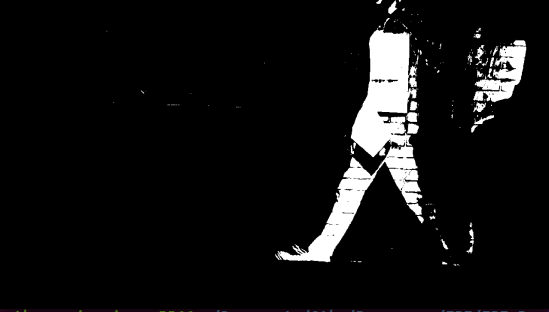
\includegraphics[scale=0.5]{background_sub.png}}
	\caption{An pedestrian moving in the scene}
	\label{fig}
	\end{figure}
	
	Obtained the moving objects from the scene, the HOG(histogram of oriented gradients) is performed in each frame from the video by an built-in function and, along with a pre-trained SVM(support vector machine) to classify human, the moving objects whose shape matches with the human shape are candidates of tracking in the process of detect pedestrian. This process is possible with the comparisson of the descriptors that the HOG provides from a window of the image(process repeated along the entire frame and for each scene) with the information that the SVM learned to classify shapes.	
	
	Once its model provide a set of the frame's regions that SVM classify as human, its possible that in the same region of a pedestrian more than one subregion is detected as human shape, and as consequence, more than one rectangle detection is marked around the person( a event observed in Figure 2).
	
	\begin{figure}[htbp]
	\centerline{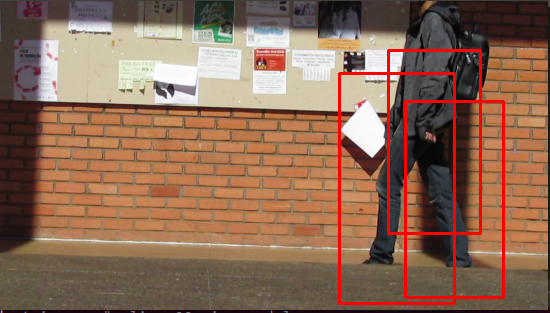
\includegraphics[scale=0.5]{Non_max.png}}
	\caption{More than one tracking in one person}
	\label{fig}
	\end{figure}
	
	For correct this kind of error, a nonmax supression built-in function was used for to reduce this redundancy tracking error. This algorithm basically get every bounding boxes that surrounds human shape compare its ratio of overlapping between then, and being a thresh ratio set, every boxes that share a ratio bigger than the overlap thresh is supressed from the region. Therefore, only sufficient distant bounding boxes will appear in the pedestrian detection.

\section{Experimental results}

\section{Conclusion}

\begin{thebibliography}{00}
\bibitem{b1} Xin Zhang, Yuehua Gao, Xiaotao Wang, Jianing Li, Bing Wang, \textit{Method for Detecting Pedestrians in Video}, 2012 International Conference on Systems and Informatics (ICSAI 2012) 
\bibitem{b2} P. KaewTraKulPong and R. Bowden ,\textit{An Improved Adaptive Background Mixture Model for Real-
time Tracking with Shadow Detection}, In Proc. 2nd European Workshop on Advanced Video Based Surveillance Systems, AVBS01. Sept 2001.
\bibitem{b3} N. Dalal and B.Triggs, \textit{Histograms of Oriented Gradients for Human Detection}, INRIA Rhône-Alps, 655 avenue de l’Europe, Montbonnot 38334, France 
\bibitem{b4} CHRISTOPHER J.C. BURGES , \textit{A Tutorial on Support Vector Machines for Pattern Recognition}
\bibitem{b5}
\bibitem{b6} 
\bibitem{b7} 
\end{thebibliography}
\vspace{12pt}
\end{document}
